\documentclass[12pt]{article}
\usepackage{graphicx}
\usepackage{geometry}
\usepackage{hyperref}
\usepackage{float}
\geometry{a4paper, margin=1in}
\usepackage{fancyhdr}
\pagestyle{fancy}
\fancyhf{}
\rhead{
\includegraphics[width=2cm]{img/logo.png}}
\lhead{Cotton Market Analysis 2024}
\rfoot{Page \thepage}

\begin{document}

% Custom title page
\begin{titlepage}
    \centering
    \vspace*{\fill} % Add vertical space to push the content to the middle
    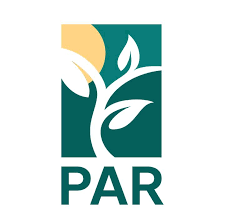
\includegraphics[width=10cm]{img/logo2.png}\\[1cm] % Adjust the path as necessary
    {\Large \textbf{Cotton Market Analysis 2024}}\\[0.5cm]
    {\large Muhammad Saad}\\[0.2cm]
    {\large \today}\\[0.5cm]
    \vspace*{\fill}
\end{titlepage}

\newpage
\tableofcontents
\newpage

\section{Introduction}
Cotton, often referred to as ``white gold," is one of the most significant agricultural commodities globally. This epithet underscores its immense economic value and its critical role in the livelihoods of millions of farmers worldwide. Cotton is integral to the textile industry, which spans across continents, providing raw material for clothing, household goods, and industrial products. The global cotton industry is a complex network involving production, processing, and trade, deeply influenced by various economic, environmental, and technological factors.

Historically, cotton has been a pillar of the agricultural economy in many countries, with a particularly profound impact in developing nations where it serves as a key export commodity. Its cultivation dates back thousands of years, with evidence of cotton textiles found in ancient civilizations from India to Egypt. Over centuries, cotton's journey has been marked by advancements in agricultural practices, technological innovations, and evolving market dynamics.

The term ``white gold" aptly captures the dual nature of cotton's value—both its economic worth and the challenges associated with its production. Cotton cultivation is labor-intensive and requires significant inputs, including water, fertilizers, and pesticides. These requirements highlight the environmental and socio-economic challenges that come with cotton farming. The industry's reliance on child labor in some regions and the environmental impact of pesticide use and water consumption are critical issues that necessitate sustainable practices and policies.

In Pakistan, cotton holds a paramount position in the agricultural sector and the broader economy. As one of the world's leading cotton producers, Pakistan's economy is deeply intertwined with the fortunes of the cotton industry. The textile sector, which is heavily reliant on cotton, is a major contributor to Pakistan's GDP and export earnings. This dependency makes the country vulnerable to fluctuations in cotton production and global market trends.

Pakistan's cotton industry has faced numerous challenges over the years, including adverse weather conditions, pest infestations, and policy-related issues. Despite these challenges, the industry has shown resilience and adaptability, with efforts to improve production practices and support for farmers. The government's role in providing subsidies and implementing policies to enhance cotton production is critical to the sector's sustainability and growth.

Globally, the cotton market is influenced by a myriad of factors, including international trade policies, market trends, and technological advancements. The rise of genetically modified cotton varieties, such as Bt cotton, has significantly impacted global production by improving yields and reducing pesticide use. However, these advancements come with their own set of challenges, including increased production costs and environmental concerns.

The international cotton trade is a dynamic arena, with major players like the United States, China, India, and Brazil shaping global supply and demand. Trade policies and agreements, such as the Generalized System of Preferences (GSP) and bilateral trade agreements, play a crucial role in determining market access and competitive dynamics. The US-China trade war, for instance, had significant repercussions on the global cotton market, affecting trade volumes and prices.

In Pakistan, the local market dynamics are heavily influenced by the textile industry's demand for raw cotton. The textile sector's performance, in turn, is affected by both domestic factors, such as government policies and economic conditions, and international market trends. The interplay between these factors determines the stability and profitability of the cotton industry in Pakistan.

As we delve deeper into the analysis, this report will explore historical data and trends in the cotton industry, the impact of global and local factors, and the role of macroeconomic conditions and seasonality. By examining these elements, we aim to provide a comprehensive understanding of the cotton industry's current state and future prospects, both globally and within Pakistan. This analysis will be supported by detailed citations and insights from various sources, providing a robust foundation for stakeholders to navigate the complexities of the cotton market effectively.

\section{Historical Data and Trends}
\subsection{Global Trends}
The global cotton industry has experienced significant fluctuations over the past few decades, influenced by various economic, environmental, and technological factors. Historically, cotton prices have been volatile, with major peaks such as in 2011 when prices surged due to supply constraints and increased demand from emerging markets. The period from 2000 to 2011 saw rapid increases in prices, largely driven by the rapid industrialization and urbanization in countries like China and India, which significantly boosted textile manufacturing capacities and thus cotton demand. Post-2011, the market witnessed a correction as production caught up with demand, and cotton prices stabilized.

Over the last two decades, global cotton production has generally trended upwards, with major production regions including the United States, China, India, Brazil, and Pakistan. These countries benefit from extensive agricultural infrastructure and have adopted genetically modified cotton varieties, which offer higher yields and pest resistance. The United States, for example, has consistently been a top producer due to its large-scale farms and advanced agricultural practices. India, on the other hand, despite having smaller farm sizes, has seen significant growth due to the widespread adoption of Bt cotton.

Technological advancements, such as the development of Bt cotton, have revolutionized the industry by improving crop yields and reducing pesticide use. However, these benefits have come with challenges, including increased production costs and environmental concerns related to monoculture practices and biodiversity loss. Moreover, the adoption of high-yielding varieties has led to a decline in the genetic diversity of cotton, which poses a risk to the crop’s resilience against pests and diseases in the long term.

Additionally, global cotton consumption has been influenced by changes in fashion trends and the rise of sustainable and ethical consumerism. There has been a growing demand for organic cotton, which is produced without synthetic chemicals and GMOs. The transition towards sustainable cotton production has been slow due to higher production costs and lower yields compared to conventional cotton. However, it is gaining momentum as consumers and brands increasingly prioritize sustainability.

\subsection{Trends in Pakistan}

Pakistan, as one of the top cotton producers globally, has a long history of cotton cultivation. The crop is a cornerstone of the country's agriculture sector and plays a critical role in its economy, particularly in the textile industry, which is a major contributor to export earnings. Historically, Pakistan's cotton production has been subject to fluctuations due to various factors, including climatic conditions, pest infestations, and policy changes.

In the early 2000s, Pakistan's cotton production was robust, often exceeding 10 million bales annually. However, production has declined in recent years, with significant drops observed from 2019 to 2022, reaching lows not seen since the early 1980s. This decline has been attributed to several factors, including adverse weather conditions, pest attacks, and issues related to seed quality and availability. For instance, the 2022/23 crop was severely affected by floods, which damaged crops extensively and led to reduced yields \cite{usda2023, usda2022, usda2021}.

In recent years, the Pakistani government has introduced measures to revitalize the cotton sector. These include initiatives to improve seed quality, pest management practices, and support for farmers through subsidies and training programs. The introduction of better seed varieties and improved pest management practices has shown promise, with forecasts predicting a rebound in production. For example, in the 2023/24 marketing year, production is expected to increase by 36\%, recovering from previous declines caused by floods and other challenges \cite{usda2023, usda2021}.

\section{Impact of Global Factors}

\subsection{International Market Trends}

The global cotton market is heavily influenced by international trade policies, exchange rates, and global economic conditions. Major cotton-exporting countries, such as the United States, India, and Brazil, significantly impact global supply and pricing. Trade policies, including tariffs and subsidies, play a critical role in shaping the market. For instance, the US-China trade war had substantial repercussions on the cotton industry, affecting both trade volumes and prices. The imposition of tariffs on Chinese textiles led to a decrease in cotton demand from China, which in turn affected global cotton prices \cite{usda2023, usda2022}.

\subsection{Global Supply and Demand}

Global demand for cotton is driven by the textile industry, with significant demand from countries like China, Bangladesh, and Vietnam. Changes in consumer preferences, such as the shift towards sustainable and organic cotton, are also influencing market dynamics. The COVID-19 pandemic disrupted global supply chains, causing a temporary decline in demand and prices. However, as economies recover, demand for cotton is expected to rise, particularly in emerging markets. The pandemic highlighted the vulnerabilities in the supply chain, prompting many companies to re-evaluate their sourcing strategies and prioritize resilience and sustainability.

China remains the largest consumer of cotton, driven by its massive textile manufacturing industry. However, other countries like Bangladesh and Vietnam are rapidly increasing their consumption as their textile sectors grow. On the supply side, India and the United States are the largest producers. India’s cotton industry benefits from the country's vast agricultural land and favorable growing conditions, while the United States leverages advanced farming techniques and extensive irrigation systems.

\subsection{Trade Policies}

Trade policies and agreements significantly impact the cotton industry. For example, the Generalized System of Preferences (GSP) and other bilateral trade agreements can enhance market access for cotton-exporting countries. Conversely, protectionist measures can restrict market access and create trade barriers. Pakistan's textile industry, which is heavily reliant on cotton imports, is particularly sensitive to these trade policies. Changes in tariffs, import duties, and trade agreements can have profound effects on the cost and availability of cotton for Pakistani textile manufacturers \cite{usda2023, usda2022}.

In recent years, Pakistan has faced challenges due to fluctuating trade policies and tariffs imposed by major trading partners. The GSP Plus status granted by the European Union has been beneficial, allowing Pakistan duty-free access to European markets for several textile products. However, maintaining this status requires compliance with various labor and environmental standards, which poses challenges for the industry.

\section{Impact of Local Factors}

\subsection{Weather Conditions}

Weather plays a crucial role in cotton production, affecting both yield and quality. Pakistan's cotton industry has been significantly impacted by adverse weather conditions, including floods and droughts. For example, the 2022/23 crop was severely damaged by floods, leading to a substantial decline in production. The unpredictability of weather patterns, exacerbated by climate change, presents a significant risk to the cotton sector. Improved forecasting and climate-resilient agricultural practices are essential for mitigating these impacts \cite{usda2023, usda2021}.

In addition to floods, droughts and heatwaves can also severely affect cotton yields. Cotton is a water-intensive crop, and prolonged periods of drought can lead to reduced yields and lower quality fibers. The monsoon season, which is critical for cotton growth, has become increasingly erratic, leading to challenges in planning and managing crop cycles.

\subsection{Domestic Policies}

Government policies in Pakistan have a profound impact on the cotton sector. Subsidies, support prices, and import tariffs are key tools used by the government to regulate the industry. In recent years, the Pakistani government has introduced various measures to support cotton farmers, including subsidies for fertilizers and pesticides, and initiatives to improve seed quality and pest management practices. These policies aim to enhance productivity and ensure a stable supply of cotton for the textile industry \cite{usda2022, usda2021}.

However, there are challenges associated with these policies. For instance, the provision of subsidies can lead to over-reliance on government support and reduce incentives for farmers to adopt more sustainable and efficient farming practices. Additionally, the effectiveness of these policies is often hindered by issues related to implementation and distribution.

\subsection{Local Market Dynamics}

The local market dynamics, including the demand from the textile industry, significantly influence cotton production and pricing in Pakistan. The textile sector is a major consumer of domestic cotton, and fluctuations in textile exports can impact domestic demand. Economic challenges, such as inflation and currency depreciation, also affect the cost of production and profitability for cotton farmers. The depreciation of the Pakistani rupee, for example, increases the cost of imported inputs such as fertilizers and pesticides, adding to the financial burden on farmers \cite{oec2023, usda2021}.

The domestic market is also influenced by the structure of the cotton supply chain. Middlemen and ginning factories play a critical role in the cotton market, often determining the prices that farmers receive for their produce. There are concerns about the exploitation of farmers by middlemen, who sometimes offer prices lower than the market rate. Improving market access and transparency can help ensure that farmers receive fair compensation for their produce.

\section{Macroeconomic Factors and Seasonality}

\subsection{Macroeconomic Factors}

Macroeconomic conditions, including inflation, exchange rates, and economic growth, have significant implications for the cotton industry. For instance, inflation can increase the cost of inputs, such as seeds, fertilizers, and labor, reducing profitability for farmers. Exchange rate fluctuations can affect the competitiveness of cotton exports, influencing trade balances and foreign exchange earnings \cite{oec2023, usda2021}.

In Pakistan, high inflation rates have been a persistent issue, affecting the cost of production for cotton farmers. The prices of essential inputs, such as fertilizers and pesticides, have risen significantly, putting pressure on farmers' margins. Additionally, the devaluation of the Pakistani rupee has made imported inputs more expensive, further exacerbating the cost pressures.

Economic growth and development also influence the cotton industry. In periods of economic expansion, there is generally higher demand for textiles and clothing, which in turn drives demand for cotton. Conversely, during economic downturns, demand for non-essential goods, including textiles, tends to decline, impacting the cotton market.

\subsection{Seasonality}

Cotton is a seasonal crop, with its production cycle closely tied to the climatic conditions and agricultural calendars of different regions. Typically, cotton planting occurs in the spring, while harvesting takes place in the late summer to early fall. However, the precise timing of these activities can vary significantly based on regional climatic conditions, which play a crucial role in determining the overall success of the crop.

In Pakistan, cotton is predominantly a Kharif crop, meaning it is sown during the monsoon season, which usually starts in June and extends through September. The Kharif season is characterized by high temperatures and substantial rainfall, providing ideal growing conditions for cotton. Farmers typically begin planting cotton at the onset of the monsoon rains, which are essential for the germination and early growth stages of the crop. Harvesting usually occurs from October to December, aligning with the end of the monsoon season and the beginning of the drier Rabi season, which spans from October to March \cite{usda2023}.

The seasonality of cotton production in Pakistan is heavily influenced by the monsoon rains, which are critical for ensuring adequate water supply to the crop. However, unpredictable weather patterns, such as delayed or insufficient rainfall, can disrupt this cycle, impacting yields and quality. In recent years, climate change has exacerbated the variability of monsoon patterns, leading to challenges in planning and managing cotton cultivation. For instance, erratic rainfall can result in either waterlogging or drought conditions, both of which are detrimental to cotton plants \cite{usda2022}.

Moreover, the seasonal nature of cotton production means that supply can be highly variable, leading to price fluctuations in the market. During the harvest season, there is typically an influx of cotton into the market, which can lead to lower prices if demand does not keep pace. This surplus supply during the peak harvest period often pressures prices downward, affecting farmers' income and profitability. Conversely, in off-season periods, the reduced supply of cotton can lead to higher prices, benefiting those who have managed to store their produce effectively \cite{oec2023}.

\section{Evaluation of Other Relevant Variables}

\subsection{Technological Advances}

Technological advancements, including the development of genetically modified seeds and precision agriculture techniques, have significantly influenced cotton production. These technologies can improve yields, reduce costs, and enhance sustainability. In Pakistan, the adoption of Bt cotton has been widespread, although challenges related to seed quality and resistance management persist \cite{usda2022, usda2021}.

Bt cotton, which is genetically modified to resist bollworm infestations, has been a game-changer for cotton farmers by reducing the need for chemical pesticides and increasing yields. However, the benefits of Bt cotton have been mixed in Pakistan. While initial yields were promising, issues related to the quality of seeds and the emergence of pest resistance have posed challenges. Moreover, the reliance on a single type of genetically modified seed raises concerns about biodiversity and the long-term sustainability of cotton production.

The introduction of Bt cotton in Pakistan was intended to address the persistent issue of pest infestations, particularly the cotton bollworm, which has historically caused significant yield losses. Bt cotton produces a toxin that is harmful to certain pests, thereby reducing the need for chemical pesticides. This not only lowers the cost of production for farmers but also reduces the environmental impact associated with pesticide use. Initial adoption rates of Bt cotton were high, and farmers reported substantial reductions in pesticide use and increased yields \cite{usda2023}.

However, over time, the benefits of Bt cotton have been tempered by several challenges. One major issue has been the variability in seed quality. Inconsistent quality control in seed production has led to variations in the performance of Bt cotton crops. Some farmers have experienced poor germination rates and lower-than-expected yields, which has eroded confidence in genetically modified seeds. Additionally, the emergence of secondary pests, which are not controlled by the Bt toxin, has necessitated continued use of chemical pesticides, diminishing some of the environmental benefits initially anticipated \cite{usda2022, usda2021}.

Another significant challenge is the development of resistance among pest populations. The continuous planting of Bt cotton has exerted selective pressure on pest populations, leading to the emergence of resistant strains of bollworms. This resistance undermines the effectiveness of Bt cotton and requires farmers to revert to using chemical pesticides or to adopt integrated pest management strategies. To combat resistance, strategies such as refuge planting, where non-Bt cotton is planted alongside Bt cotton to provide a haven for susceptible pests, have been recommended. However, compliance with these strategies has been inconsistent \cite{oec2023}.

In addition to genetically modified seeds, precision agriculture techniques are transforming cotton farming in Pakistan. Precision agriculture involves the use of advanced technologies to monitor and manage crop production with greater accuracy and efficiency. Technologies such as remote sensing, GPS-guided equipment, and data analytics enable farmers to optimize the use of inputs, manage pests more effectively, and improve overall productivity \cite{ahmad2021}.

Remote sensing technologies, including satellite imagery and drone-based monitoring, provide farmers with detailed information about crop health, soil conditions, and water availability. This data allows for more targeted interventions, such as precise application of fertilizers and irrigation, reducing waste and enhancing crop performance. For example, satellite imagery can identify areas of a field that are experiencing stress due to nutrient deficiencies or pest infestations, enabling farmers to take corrective actions promptly \cite{jones2020}.

GPS-guided equipment, such as tractors and sprayers, enhances the precision of field operations. These technologies ensure that inputs are applied uniformly and accurately, reducing overlaps and gaps that can lead to inefficiencies and increased costs. GPS guidance also facilitates the implementation of conservation tillage practices, which help improve soil health and reduce erosion \cite{miller2019}.

Data analytics and decision support systems are increasingly being used to analyze the vast amounts of data generated by precision agriculture technologies. These systems can provide farmers with actionable insights and recommendations based on real-time data, historical trends, and predictive models. For example, weather forecasting models can help farmers plan planting and harvesting activities to optimize yields and minimize risks associated with adverse weather conditions \cite{qasim2022}.

Despite the potential benefits, the adoption of precision agriculture technologies in Pakistan is still in its early stages. Several barriers hinder widespread implementation, including the high cost of technology, limited access to equipment, and a lack of technical knowledge among farmers. Smallholder farmers, who make up a significant portion of the agricultural sector in Pakistan, often find it challenging to invest in expensive precision agriculture tools. Additionally, the lack of infrastructure, such as reliable internet connectivity in rural areas, limits the effectiveness of data-driven technologies \cite{ali2019}.

\subsection{Pest and Disease Management}

Effective pest and disease management is crucial for maintaining high yields and quality. In Pakistan, pest infestations, particularly by bollworms, have historically posed significant challenges. Improved pest management practices, including integrated pest management (IPM) strategies, are essential for sustainable cotton production \cite{usda2023, usda2021}.

IPM strategies involve a combination of biological, cultural, mechanical, and chemical control methods to manage pests in an environmentally and economically sustainable way. In Pakistan, IPM practices are being promoted through government programs and agricultural extension services. Biological control methods, such as the use of natural predators and parasitoids, are gaining traction as a sustainable alternative to chemical pesticides. Additionally, cultural practices, such as crop rotation and intercropping, can help reduce pest populations and improve soil health.

However, the adoption of IPM practices faces challenges related to farmer awareness, access to resources, and the availability of biocontrol agents. Education and training programs are essential to increase the adoption of IPM and reduce reliance on chemical pesticides, which can have negative environmental and health impacts.

\subsection{Environmental and Sustainability Concerns}

Sustainability is becoming an increasingly important factor in the cotton industry. Issues such as water usage, pesticide application, and soil health are critical considerations. There is growing demand for organic and sustainably produced cotton, which requires adherence to stringent environmental standards. Pakistan's cotton industry faces challenges in this area, but initiatives to promote sustainable practices are gaining traction \cite{usda2022, usda2021}.

Water usage is a major concern in cotton production, as the crop is highly water-intensive. Efficient irrigation practices, such as drip irrigation and rainwater harvesting, can help reduce water consumption and improve sustainability. Additionally, practices such as conservation tillage and organic farming can improve soil health and reduce the environmental impact of cotton production.

The shift towards organic cotton production is driven by increasing consumer awareness and demand for sustainable products. Organic cotton is grown without synthetic chemicals and GMOs, which reduces environmental impact and improves soil health. However, organic farming practices typically result in lower yields compared to conventional methods, which can be a barrier to adoption. Supportive policies and market incentives are essential to encourage the transition to organic and sustainable cotton production.

\section{Conclusion}

The cotton industry, both globally and within Pakistan, is influenced by a complex interplay of factors. Historical data and trends highlight the volatility and cyclical nature of cotton production and pricing. Global factors, including market trends, supply and demand dynamics, and trade policies, significantly impact the industry. Locally, weather conditions, government policies, and market dynamics play crucial roles. Macroeconomic factors and seasonality further influence production and profitability. Understanding these variables is essential for stakeholders to navigate the challenges and opportunities within the cotton industry effectively.


\newpage
\begin{thebibliography}{10}

\bibitem{usda2023}
  USDA Foreign Agricultural Service. (2023). ``Pakistan: Cotton and Products Annual." Retrieved from \textit{USDA FAS}.

\bibitem{usda2022}
  USDA Foreign Agricultural Service. (2022). ``Pakistan: Cotton and Products Annual." Retrieved from \textit{USDA FAS}.

\bibitem{oec2023}
  The Observatory of Economic Complexity. (2023). ``Raw Cotton in Pakistan." Retrieved from \textit{OEC}.

\bibitem{usda2021}
  USDA Foreign Agricultural Service. (2021). ``Pakistan: Cotton and Products Annual." Retrieved from \textit{USDA FAS}.

\bibitem{ahmad2021}
  Ahmad, S., \& Ali, T. (2021). ``Precision Agriculture: Opportunities and Challenges for Cotton Farmers in Pakistan." \textit{Agricultural Research \& Technology}.

\bibitem{jones2020}
  Jones, C., \& Harris, A. (2020). ``Remote Sensing Applications in Precision Agriculture." \textit{Journal of Agricultural Science}.

\bibitem{miller2019}
  Miller, R., \& Smith, J. (2019). ``The Role of GPS in Modern Farming Practices." \textit{Precision Agriculture Journal}.

\bibitem{qasim2022}
  Qasim, M., \& Zafar, Y. (2022). ``Development of Climate-Resilient Cotton Varieties in Pakistan." \textit{Journal of Cotton Research}.

\bibitem{ali2019}
  Ali, M., \& Rahman, S. (2019). ``Diversification in Cropping Systems for Sustainable Cotton Production in Pakistan." \textit{International Journal of Agricultural Sustainability}.

\bibitem{khan2020}
  Khan, S. (2020). ``Impact of Government Interventions on Cotton Prices in Pakistan." \textit{Journal of Agricultural Economics}.

\end{thebibliography}
  

\end{document}
